\chapter{Choosing Transformer-based Toxicity Analyzer} \label{choosing-toxicity-analyzer}
To predict the toxicity of toots, we evaluated three models: Detoxify (Original), Detoxify (Unbiased) from Unitary, and Perspective API. These models predict probabilities for six to seven toxicity categories.

\section{Mastodon Posts Annotation} \label{annotation}
All models were evaluated on a subset of the dataset. The selected timeframe was the evening of the 2024 Paris Olympic Games' opening ceremony, chosen due to the expectation of heightened online discussions and increased toxic content. The dataset covers the period from 20:00 to 23:00 on July~26, 2024, comprising 1,179,897 toots. This context switch may impact model performance but also demonstrates robustness in a new context.

After predictions were completed, a sample was drawn for each model, selecting 25 toots per toxicity category with a predicted probability greater than 0.5. The selected toots were concatenated, and duplicates were removed, resulting in a final annotation dataset of 253 toots.

Two researchers conducted the annotation process using Label Studio. The toots were labeled according to the categories in Table~\ref{toxicity-categories}. Hate speech annotation is highly subjective and influenced by annotator biases, affecting consistency and reliability. To ensure reliability, inter-annotator agreement was measured using Cohen's Kappa. The results showed perfect agreement (Cohen's Kappa = 1.0) for the categories toxic, severe toxic, threat, insult, and identity attack. Near-perfect agreement was achieved for obscene (Cohen's Kappa = 0.9907) and sexually explicit (Cohen's Kappa = 0.9735), indicating high consistency between annotators.

\begin{table}[tb]
    \centering\small
    \renewcommand{\arraystretch}{1.3}
    \begin{tabularx}{\textwidth}{lX}
        \toprule
        \textbf{Category} & \textbf{Description} \\
        \midrule
        TOXIC & A rude, disrespectful, or unreasonable comment that is likely to make someone leave a discussion. \\
        SEVERE TOXIC & A very hateful, aggressive, or disrespectful comment that is highly likely to push someone away. \\
        IDENTITY ATTACK & Negative or hateful comments targeting someone because of their identity. \\
        INSULT & Insulting, inflammatory, or negative comments towards a person or group. \\
        OBSCENE & Swear words, curse words, or other obscene or profane language. \\
        THREAT & Describes an intention to inflict pain, injury, or violence against an individual or group. \\
        SEXUALLY EXPLICIT & Genital nudity or descriptions of simulated or actual sexual acts. \\
        \bottomrule
    \end{tabularx}
    \caption{Toxicity Categories and Their Descriptions}
    \label{toxicity-categories}
\end{table}

\section{Transformer-based Model Evaluation} \label{evaluation}
The evaluation focused on the probability distributions of toxicity categories and the F1 scores across the three models: Perspective API, Detoxify (Original), and Detoxify (Unbiased). The F1 score, calculated as:

\[
F1 = 2 \times \frac{\text{precision} \times \text{recall}}{\text{precision} + \text{recall}},
\]

was used to measure prediction performance, as it balances precision and recall.

A fixed threshold of 0.5 was used to compare F1 scores. The Perspective API model generally outperformed the Detoxify models in F1 scores for most categories (see Table~\ref{table-performance-metrics}). However, the probability distributions (Figure~\ref{probability-distribution}) revealed behavioral differences. The Perspective API model exhibited a widely spread distribution, suggesting cautious predictions, while the Detoxify models showed concentrated distributions, indicating higher confidence.

\begin{figure}[tb]
    \centering
    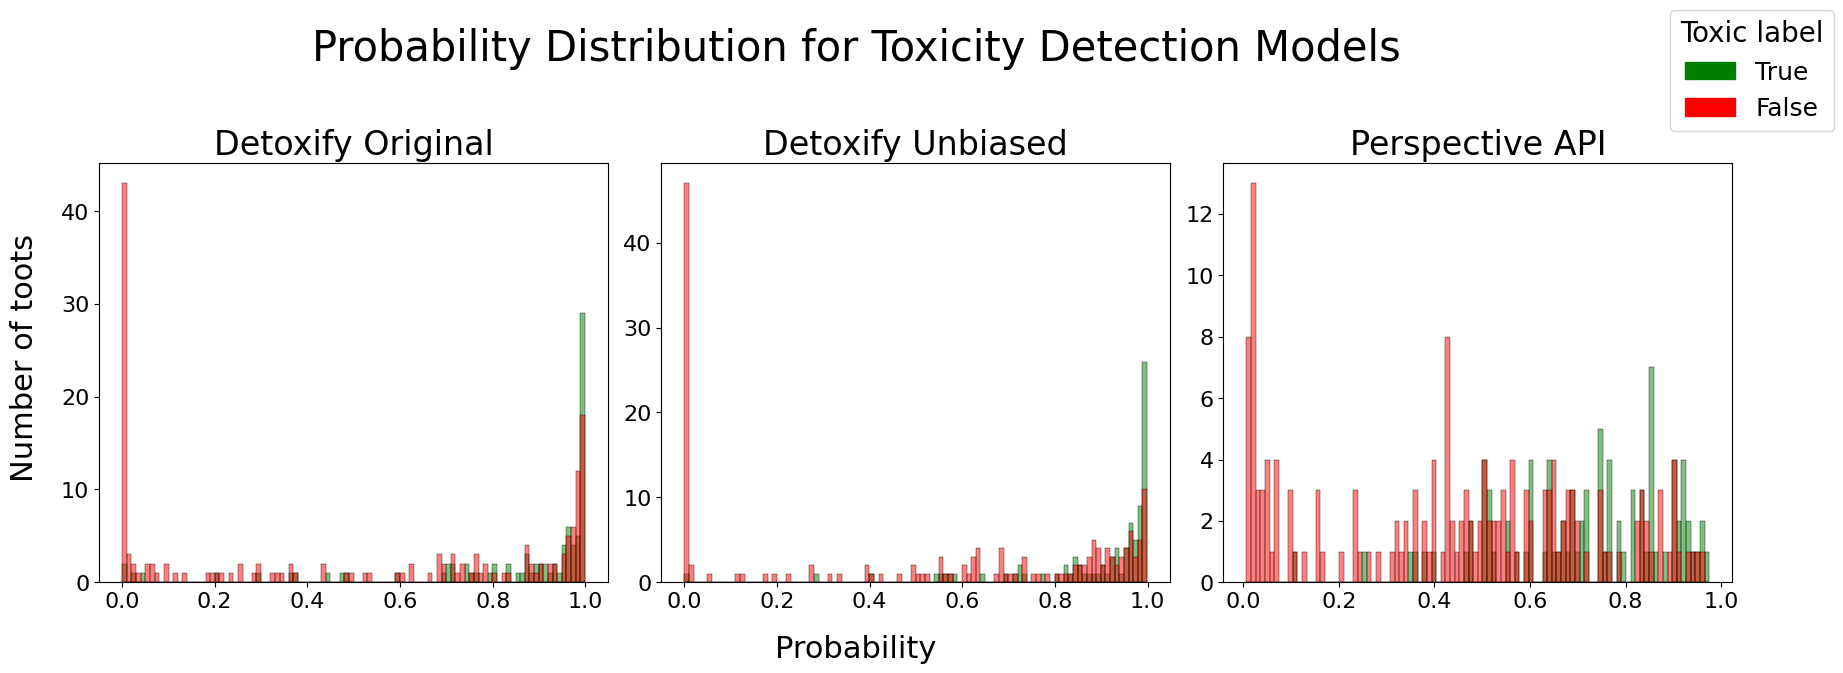
\includegraphics[width=\textwidth]{../material/probability_distribution.png}
    \caption{Probability Distribution of Toxicity category across the three models}
    \label{probability-distribution}
\end{figure}

The Perspective API model's limited accessibility, due to low request rates and lack of open access, posed practical constraints for large-scale analysis. In contrast, the open-source Detoxify models offered unrestricted usage, making them more suitable for extensive studies. Since the research goal is to analyze broader toxicity trends rather than individual toots, the Detoxify models were deemed more appropriate. A confident model like Detoxify is better for tracking trends over time.

Between the two Detoxify models, the unbiased version was selected for further analysis due to its superior performance (Table~\ref{table-performance-metrics}) and inclusion of the "sexual explicit" category, absent in the original model. However, the "severe toxic" label in the unbiased model performed poorly, likely due to limited supporting toots (only 10 in the dataset). Findings for this category should be interpreted cautiously. Despite this, the Detoxify unbiased model was chosen for analyzing Mastodon toxicity trends, balancing performance, accessibility, and practicality.

\begin{table}[p]
    \centering\small
    \caption{Performance metrics across toxicity categories with highest F1 scores highlighted.}
    \label{table-performance-metrics}
    \begin{tabular}{@{}lrrrr@{}}
      \toprule
      \textbf{Model} & \textbf{F1} & \textbf{Precision} & \textbf{Recall} & \textbf{Support} \\
      \midrule
      \multicolumn{5}{c}{\bfseries toxic} \\
      Detoxify Original      & 0.622 & 0.482 & 0.878 & 90 \\
      Detoxify Unbiased      & 0.635 & 0.473 & 0.967 & 90 \\
      Perspective API        & \textbf{0.664} & 0.526 & 0.900 & 90 \\
      \addlinespace[0.5em]
      
      \multicolumn{5}{c}{\bfseries severe toxic} \\
      Detoxify Original      & 0.148 & 0.118 & 0.200 & 10 \\
      Detoxify Unbiased      & 0.000 & 0.000 & 0.000 & 10 \\
      Perspective API        & \textbf{0.222} & 0.176 & 0.300 & 10 \\
      \addlinespace[0.5em]
      
      \multicolumn{5}{c}{\bfseries obscene} \\
      Detoxify Original      & \textbf{0.741} & 0.613 & 0.936 & 78 \\
      Detoxify Unbiased      & 0.739 & 0.642 & 0.872 & 78 \\
      Perspective API        & 0.738 & 0.615 & 0.923 & 78 \\
      \addlinespace[0.5em]
      
      \multicolumn{5}{c}{\bfseries threat} \\
      Detoxify Original      & 0.462 & 0.429 & 0.500 & 18 \\
      Detoxify Unbiased      & 0.520 & 0.406 & 0.722 & 18 \\
      Perspective API        & \textbf{0.596} & 0.483 & 0.778 & 18 \\
      \addlinespace[0.5em]
      
      \multicolumn{5}{c}{\bfseries insult} \\
      Detoxify Original      & 0.377 & 0.312 & 0.476 & 42 \\
      Detoxify Unbiased      & \textbf{0.500} & 0.378 & 0.738 & 42 \\
      Perspective API        & 0.487 & 0.384 & 0.667 & 42 \\
      \addlinespace[0.5em]
      
      \multicolumn{5}{c}{\bfseries identity attack} \\
      Detoxify Original      & 0.440 & 0.314 & 0.733 & 15 \\
      Detoxify Unbiased      & \textbf{0.545} & 0.414 & 0.800 & 15 \\
      Perspective API        & 0.456 & 0.310 & 0.867 & 15 \\
      \addlinespace[0.5em]
      
      \multicolumn{5}{c}{\bfseries sexually explicit} \\
      Detoxify Original      & 0.000 & 0.000 & 0.000 & 21 \\
      Detoxify Unbiased      & 0.392 & 0.333 & 0.476 & 21 \\
      Perspective API        & \textbf{0.576} & 0.447 & 0.810 & 21 \\
      \bottomrule
    \end{tabular}
  \end{table}